\chapter{Dziedzina problemu}

\begin{figure}
 \centering
 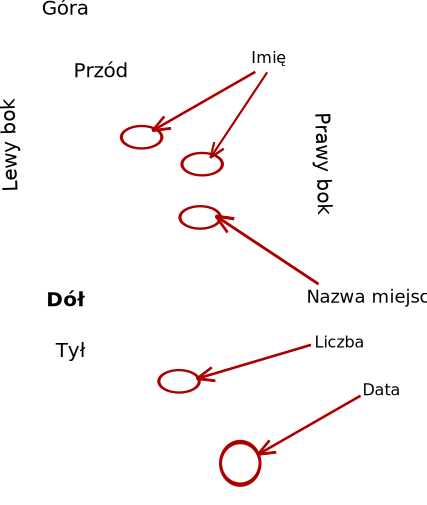
\includegraphics[bb=0 0 342 405]{../diagramy/tabliczka.pdf}
 % tabliczka.pdf: 342x405 pixel, 72dpi, 12.06x14.29 cm, bb=0 0 342 405
 \caption{Gliniana tabliczka - struktura}
\end{figure}

\begin{figure}
 \centering
 
\includegraphics[width=500px,bb=0 0 650 345]{../diagramy/Model-dziedziny.png}
 % Model-dziedziny.png: 650x345 pixel, 72dpi, 22.93x12.17 cm, bb=0 0 650 345
 \caption{Co powinna zawierać tabliczka w formie elektronicznej}
\end{figure}

Głównym pojęciem dziedziny jest tabliczka rozumiana dwojako - jako fizyczna tabliczka gliniana lub jako tabliczka w formie cyfrowej. Najważniejszym elementem tabliczki jest treść zapisana klinami w tabliczce glinanej, odczytami w tabliczce elektronicznej. Tabliczka elektroniczna zawiera także metadane informujące m. in. o jej miejscu znalezienia, czasie powstania, kolekcji do której obecnie należy.
% Ma ona swoje metadane i treść. 
%Tabliczka jest rozumiana dwojako - jako fizyczna tabliczka gliniana zapisana klinami lub jako tabliczka w formie cyfrowej zapisana odczytami. 
Treść tabliczki może zawierać elementy znaczące, takie jak imię 
osoby, imię bóstwa, liczba, jednostka (np. przy opisywaniu wypłat), miejsce, data. Część tych elementów można przetłumaczyć na 
współczesny język (np. jednostki przeliczyć na SI, datę opisową na datę liczbową BC). Gliniane tabliczki są zapisywane z różnych stron 
(od góry, z przodu, z tyłu itp), zawierają też pieczęcie - co znajduje odzwierciedlenie w treści tabliczki elektronicznej. 

Odczyty zawarte w cyfrowym zapisie tabliczki są wariantem tłumaczenia z klinów. W cyfrowej wersji nie ma klinów, stąd też możliwe
są pomyłki w tłumaczeniach, które ciężko zweryfikować. Są też uszkodzone fragmenty, które zostały cyfrowo zapisane w najróżniejszej
formie.


%TODO:spytać
Sumerolodzy potrafią określić w przybliżeniu treść tabliczki na podstawie publikacji.
%TODO::ciągłość

Sumerolodzy oczekują możliwości wyszukiwania po metadanych, po treści tabliczki (odczyty) i po możliwych innych tłumaczeniach (po klinach). Dodatkowym plusem byłoby wyszukiwanie po tagach (ludziach, jednostkach, datach itp)
W pierwszej wersji języka implementujemy tylko wyszukiwanie po odczytach i metadanych.